\chapter[SCP-160 掠食无人机]{
    SCP-160 Predator Drone\\
    SCP-160 掠食无人机
}

\label{chap:SCP-160}

\begin{figure}[H]
    \centering
    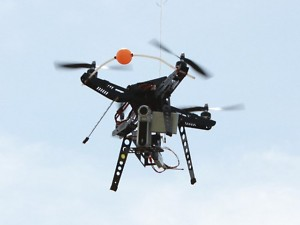
\includegraphics[width=0.5\linewidth]{images/SCP.160.jpg}
    \caption*{初步收容时的SCP-160}
\end{figure}

\bb{项目编号:}SCP-160

\bb{项目等级:}Euclid

\bb{特殊收容措施:}SCP-160保存在██处的一个安全的生物保存室当中,SCP-160每周需喂食一次如兔子或者其它类似大小的动物等活体猎物。喂食必须完全由自动供应系统完成。

对SCP-160进行的实验需要得到至少两名3级成员的许可才可以进行,进入保存室的人员必须全程穿戴防护盔甲。

\bb{描述:}SCP-160的外观是一架标准的无人机(UAV),翼展最宽处直径1.1m,和{[}删除]公司生产的{[}删除]型号相类似。其机体上没有任何身份标示和生产标签,尽管通过外观可以观测到SCP-160上面的的划痕和表面损伤可以推测先前的身份标签已被除去。

SCP-160保持着持续的运转并且完全不受任何可确认的控制源影响,并且它的习性和猛禽非常类似。它会主动“猎捕”诸如松鼠和其它小型动物之类的猎物,并且在发现此类猎物之后,会以高速俯冲下来并用一根类似于金属吸管的装置刺穿猎物。对猎物的分析显示它会向猎物注入一种高度腐蚀性的物质液化猎物的内部器官,然后吸取猎物的体液。SCP-160一般会躲避人类和大型的动物,但是记录显示它也会使用它的捕食装置进行自卫。被SCP-160“咬伤”会导致极度疼痛,并且会由于重要器官液化和内出血导致死亡。

对SCP-160的进一步研究还在进行当中,但是由于SCP-160的持续运转使得这变得非常困难。由于SCP-160看起来完全是由无机材料构成所以镇静剂飞镖没有作用,而使用低强度电磁波将其关闭的提案由于考虑到可能造成不可预知的损害而被拒绝。

SCP-160被一名基金会的特工发现于█\slash ██\slash 200█由于接到了{[}删除]小镇的数起家养宠物失踪事件报告。SCP-160被迅速的鉴定并被抑制小组引诱进一辆运输车内送往██地点。通过对区域内的进一步搜索发现了很多脱水小动物的尸体,包括家猫,兔子,松鼠和小型犬等等。
